%\chapter{Implementación del código numérico en GPU}
\chapter{Código numérico de LBM en GPU}
\graphicspath{{figs/cap3/}}
\label{cap3}



%\section{Implementación del código}

En el presente capítulo se realizará la descripción de la implementación del código numérico del LBM descripto en la Sec. (\ref{sec:LBM_2_ec_MRT}); como también las implicancias de elaborar la implementación en una GPU de forma eficiente.

El lenguaje de programación \textbf{C} desarrollado por Dennis MacAlistair Ritchie será utlizado primeramente para confeccionar el código. Dicho lenguaje brinda instrucciones a la CPU de una PC para ser ejecutadas. Las CPU son diseñadas óptimamente para que sus instrucciones sean procesadas de forma secuencial en los núcleos que poseen; aunque también se permite realizar los procesos en paralelo, según la cantidad de núcleos.

Luego se implementará un código en \textbf{CUDA C} el cuál fue desarrollado por la empresa NVIDIA. Este lenguaje permite ejecutar instrucciones en una GPU, la cuál está diseñada para que los procesos a realizar sean de forma paralela.

Ambos códigos , \textbf{C} y \textbf{CUDA C}, son compilados en bibliotecas estáticas mediante \textbf{CMake}. Con las bibliotecas compiladas se prosigue a utilizarlas mediante el lenguaje de programación interpretado \textbf{Python}. La bibliotecas necesarias para que el código de \textbf{C} y \textbf{CUDA C} puedan ser llevadas a cabo en \textbf{Python} son \textit{CTypes} y \textit{PyCUDA} respectivamente.

Se eligió la programación en \textbf{C} y \textbf{CUDA C} para comparar la eficiencia en el tiempo de cálculo, debido a que el lenguaje \textbf{CUDA C} es una extensión del lenguaje \textbf{C}. La diferencia principal es que \textbf{CUDA C}  tiene una forma particular de escribir las funciones que se ejecutarán en la GPU, las cuáles son llamadas \textit{kernel}.

La implementación en \textbf{Python} es debido a su facilidad de programación, el cuál permite incorporar las bibliotecas compiladas y obtener una mayor versatilidad de problemas a resolver. \textbf{Python} puede ser utilizado en distintos sistemas oparativos como \textit{Linux}, \textit{Windows} y \textit{Mac OS}. 

En \textbf{Python} sólo se realizará la implementación con la biblioteca \textit{PyCUDA}, debido a que se espera una mayor eficiencia en tiempos de cálculo que en \textit{CTypes}.




\section{Programación en GPU}

Una computadora (\textit{Personal Computer} o PC) posee como procesador principal la CPU, cuyo diseño se encuentra optimizado para realizar tareas secuenciales. Comercialmente vienen de una amplia variedad de núcleos, en el rango de 8 a 64 núcleos en el caso de los Procesadores AMD Ryzen™ Threadripper, 4 a 8 núcleos en los Procesador AMD FX™, en el caso de Intel se encuentra el Procesador Intel® Core™ serie X con 18 núcleos y  Intel® Core™ I3-9100T de 4 núcleos entre otros. \cite{edp:2020:amd} \cite{icp:2020:intel}

Es posible realizar tareas y procesos en paralelo en la CPU proveyendo instrucciones a cada núcleo del procesador de forma independiente, siendo más eficiente en el tiempo de ejecución de los procesos realizados.

A su vez una PC opcionalmente puede contener un coprocesador siendo una GPU. Dicha placa se encuentra diseñada para realizar operaciones en paralelo, realizándolas en varios hilos de ejecución (\textit{threads}).




El procesador principal que tiene una PC es la CPU, por lo cual se denomina \textit{host}, la GPU es un coprocesador y se denomina \textit{device}. Las ejecuciones de los procesos en la CPU están diseñadas para que se efectúen de manera secuecncial, en cuánto las de la GPU en paralelo; las últimas realizándose en varios hilos de ejecución (\textit{threads}). Las operaciones en paralelo que son analizadas por la CPU y las deriva a la GPU son llevadas a cabo mediante funciones llamadas \textit{kernel}. \textit{Host} y \textit{device} poseen su propia memoria RAM, llamadas \textit{host memory} y \textit{device memory} respectivamente. \cite{rinaldi2011modelos}

Los \textit{threads} que posee una GPU se pueden agrupar de dos formas, una de ellas es por bloques (\textit{thread block}) y la otra mediante grilla de bloques (\textit{grid}). Todos los \textit{threads} del mismo \textit{thread block} poseen un acceso rápido a una memoria compartida y permite sincronizar las ejecuciones que se les asigna. Debido a la posibilidad de sincronización de los mismos, se evita el riesgo de que varios \textit{threads} accedan de manera simultánea al mismo lugar de memoria. Un \textit{grid} es un conjunto de \textit{thread block}, en dónde las instrucciones del \textit{kernel} son paralelizadas, ésto vence la limitación de hardware del finito número de \textit{threads} por bloque. Puesto que la ejecución del proceso en los \textit{thread blocks} de un \textit{grid} pueden ser ejecutados en tiempos distintos, es necesario realizar un sincronización entre los mismos para que su comunicación sea segura y no haya conflictos\cite{tolke2010implementation}. La figura \ref{fig:block_grid_threads} muestra el concepto de \textit{grid} y \textit{thread block}.

\newpage
\begin{figure}[h!]
	\centering
	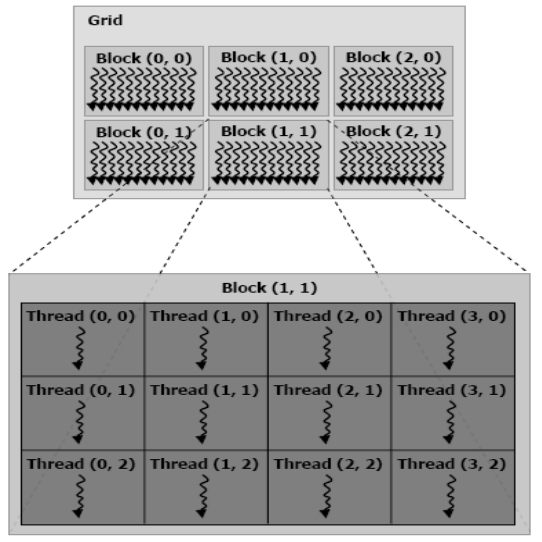
\includegraphics[width=0.4\textwidth]{figs/cap3/threads_block_grid.jpg}
	\caption{\textit{Thread blocks} organizados en un \textit{grid} \cite{rinaldi2011modelos}.}
	\label{fig:block_grid_threads}
\end{figure}



\section{Arquitectura de la memoria de una GPU}

\begin{figure}[h!]
	\centering
	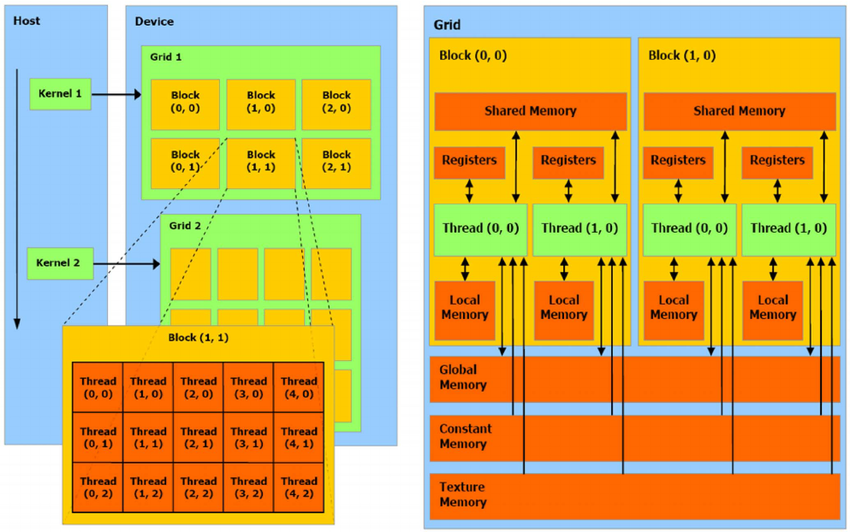
\includegraphics[width=\textwidth]{figs/cap3/Schematization-of-CUDA-architecture-Schematic-representation-of-CUDA-threads-and-memory.png}
	\caption{Esquematización de la arquitectura de CUDA. Izquierda: lanzamiento de un \textit{kernel} desde el \textit{host}. Derecha: jerarquía de memoria.  \cite{nobile2014cutauleaping}.}
	\label{fig:schedule_architecture_cuda}
\end{figure}

Según la arquitectura que posea un procesador, con su respectiva jerarquía en memoria, accesos y latencias, se planifica cómo llevar a cabo la implementación de un código, por ello es de importancia conocer dichas características. 

Anteriormente se mencionó que el \textit{host} y \textit{device} poseen su propia memoria. La transferencia de datos de una memoria a otra tiene una muy alta latencia en cualquiera de los dos sentidos; por lo que al diseñar un código, hay que minimizar la transferencia de datos entre los dos tipos de memoria, y así obtener el menor tiempo de ejecución de los procesos.

Cuando el \textit{host} efectúa su rutina de ejecución y se encuentra con un lanzamiento de \textit{kernel}, éste será llevado a cabo en múltiples \textit{threads} del \textit{device}. Una representación de ello se muestra en la figura \ref{fig:schedule_architecture_cuda}. 

Los procesos en el \textit{device} tienen almacenados los datos según una jerarquía de memoria, con su respectiva limitación de acceso que se observa en la figura \ref{fig:schedule_architecture_cuda}. Los \textit{threads} pueden acceder a datos de muchas memorias diferentes en distintos procesos, dichas memorias son las siguientes:

\begin{itemize}
	\item  \textit{register memory} es visible para un único \textit{thread}
	\item \textit{local memory} tiene las mismas caracteísticas que \textit{register memory} pero con una performance menor.
	\item \textit{shared memory} es visible por todos los \textit{threads} de un mismo bloque, posee una baja latencia en su acceso.
	\item \textit{global memory} es visible por todos los \textit{threads} de la grilla y también por el \textit{host}, posee una alta latencia de acceso.
	
	Las siguientes memorias poseen una alta latencia de acceso son asignadas y son aignadas para usos específicos y generalmente se almacenan en \textit{caché}:
	
	\item \textit{constant memory} es visible por todos los \textit{threads} de la grilla siendo únicamente de lectura. El uso de ésta memoria puede reducir el ancho de banda de memoria requerido en comparación con la {global memory}
	\item \textit{texture memory} es otra memoria en la que sólo se puede leer y tienen acceso todos los \textit{threads} de la grilla. Al realizar lecturas de \textit{threads} ó \textit{threadblocks} adyacentes su performance en comparación con \textit{global memory} es mayor. 
	
\end{itemize}

\newpage

\section{Programación en CUDA C}

La programación de las GPU se lleva a cabo mediante el lenguaje \textbf{CUDA}, el cuál es una extención del lenguaje \textbf{C} debido su familiaridad y uso extendido; por lo que el lenguaje se denomina \textbf{CUDA C}. La realización de procesos en paralelos es ejecutada mediante funciones llamadas \textit{kernel} y son del tipo \textit{void}.
\\

Existen tres tipos de funciones que se pueden efectuar en \textbf{CUDA C} y son:

\begin{itemize}
	
	\item \textbf{host} función clásica de C que se ejecuta en la CPU, siendo invocable únicamente por funciones que se realicen en la CPU. 

	\item \textbf{global} es una función \textit{kernel} invocada desde la CPU para ejecutarse en la GPU. 
%	Debe especificar la cantidad de bloques y de \textit{threads} por bloque a lanzar la función.
	
	\item \textbf{device} es una función que se ejecuta en la GPU y únicamente puede ser llamada desde un \textit{kernel}.
	
\end{itemize}

En el presente trabajo sólo se utilizaran funciones de tipo \textbf{host} y \textbf{global}, pudiéndose realizar en un futuro el  \textit{profiling} mediante el uso de las funciones tipo \textbf{device}.

Otra particularidad que se presenta en la programación es el manejo de la memoria por parte del \textit{host} como del \textit{device}, siendo abordado posteriormente.


\subsection{Programación de un \textit{kernel}}

Para visualizar las diferencias de programación de una función \textbf{CUDA C } (\textit{kernel}), con una típica función de \textbf{C}, se muestra a continiación como ejemplo la programación para ambos lenguajes de la Ec. (\ref{eq:rho}): 

\begin{align*}
	\rho = \sum_{\alpha} f_{\alpha}
\end{align*}

Primeramente se detalla el código realizado en el lenguaje \textbf{C}, siendo la función :

{\footnotesize
	\begin{frame}{}
		\lstset{language=C,
			framesep=2mm,
			basicstyle=\ttfamily,
			keywordstyle=\color{blue}\ttfamily,
			stringstyle=\color{red}\ttfamily,
			commentstyle=\color{green}\ttfamily,
			morecomment=[l][\color{magenta}]{\#}
		}
		\begin{lstlisting}
void momentoDensity(scalar* rho, scalar* field, basicMesh* mesh);
		\end{lstlisting}
		
	\end{frame}
}.
\\
donde el argumento \textbf{basicMesh* mesh} es un puntero a una estructura, la cuál posee información del mallado que se realizó al dominio del problema a resolver ; como por ejemplo la cantidad de nodos que posee la malla (\textbf{nPoints}) y la cantidad de direcciones que posee el modelo en su espacio de velocidades \textbf{Q}. El vector  \textbf{scalar* rho} es de dimensión \textit{nPoints} y contiene los valores de $\rho$, por último \textbf{scalar* field} es un vector que posee las \textit{Q} componentes de la función de distribución de poblaciones \textit{f} para cada uno de los  \textit{nPoints} nodos de la malla.

Cabe destacar que los resultados obtenidos durante la programación del código en \textbf{C}, se concluyó que es más eficiente el uso de la función \textcolor{blue}{\textbf{for}} que \textcolor{blue}{\textbf{while}}.


{\footnotesize
	\begin{frame}{}
		\lstset{language=C,
			framesep=2mm,
			basicstyle=\ttfamily,
			keywordstyle=\color{blue}\ttfamily,
			stringstyle=\color{red}\ttfamily,
			commentstyle=\color{green}\ttfamily,
			morecomment=[l][\color{magenta}]{\#}
		}
		\begin{lstlisting}[frame=single]
#include <momentoDensity.h>
#include <stdio.h>

void momentoDensity(scalar* rho, scalar* field, basicMesh* mesh) {
	
	// Suma de todas las componentes
	
	for( uint i = 0 ; i < mesh->nPoints ; i++ ) {
		
		rho[i] = 0;	    
		
		for( uint j = 0 ; j < mesh->Q ; j++ ) {
		
			rho[i] += field[ i*mesh->Q + j ];
		
		}	
			
	}
	
}
		\end{lstlisting}
		
	\end{frame}
}.
\\

La programación de la Ec.(\ref{eq:rho}) implementada en \textbf{CUDA C} es con la función:

{\scriptsize
	\begin{frame}{}
		\lstset{language=C,
			framesep=2mm,
			basicstyle=\ttfamily,
			keywordstyle=\color{blue}\ttfamily,
			stringstyle=\color{red}\ttfamily,
			commentstyle=\color{green}\ttfamily,
			morecomment=[l][\color{magenta}]{\#}
		}
		\begin{lstlisting}
extern "C" __global__ void cudaMomentoDensity(cuscalar* field,
					      cuscalar* rho, int np, int Q ) ; 
		\end{lstlisting}
		
	\end{frame}
}.
\\
en éste caso se pasa de forma distinta los valores de la cantidad de nodos (\textbf{np}) y de la cantidad de velocidades del modelo \textit{DdQq} (\textbf{Q}). La distinción en los argumentos que se pasan en ambos códigos, es debido a la forma que \textbf{CUDA} permite el manejo de las estructuras y también de las decisiones que se tomaron cuando se desarrollaba el código para uno u otro lenguaje.

Se colola \textcolor{blue}{extern} \textcolor{red}{''C''} para que el compilador sepa que es una función de \textbf{CUDA} y además para que lo implemente en una biblioteca tipo \textit{ptx} para \textbf{Python}.
\newpage
{\footnotesize
	\begin{frame}{}
		\lstset{language=C,
			framesep=2mm,
			basicstyle=\ttfamily,
			keywordstyle=\color{blue}\ttfamily,
			stringstyle=\color{red}\ttfamily,
			commentstyle=\color{green}\ttfamily,
			morecomment=[l][\color{magenta}]{\#}
		}
		\begin{lstlisting}[frame=single]
#include <cudaMomentoDensity.h>
#include <cuda_runtime.h>
#include <stdio.h>
#include <stdlib.h>

extern "C" __global__ void cudaMomentoDensity(cuscalar* field,
				              cuscalar* rho,
					      int np,
					      int Q ) {
							
	int idx = threadIdx.x + blockIdx.x*blockDim.x;	
	
	if( idx < np ) {	
	
		int j= 0;		
	
		cuscalar sum = 0;		
	
		while ( j < Q ) {		
	
			sum += field[ idx*Q + j ];			
	
			j++;			
	
		}				
	
		rho[idx] = sum;	
	
	}
	
}		
		\end{lstlisting}
		
	\end{frame}
}.
\\
en éste leguaje, se observó que es más eficiente el uso de la función \textcolor{blue}{\textbf{while}} que \textcolor{blue}{\textbf{for}} en el tiempo de ejecución del código.

Es de importancia conocer la función que cumplen las siguientes líneas:
{\footnotesize
	\begin{frame}{}
		\lstset{language=C,
			framesep=2mm,
			basicstyle=\ttfamily,
			keywordstyle=\color{blue}\ttfamily,
			stringstyle=\color{red}\ttfamily,
			commentstyle=\color{green}\ttfamily,
			morecomment=[l][\color{magenta}]{\#}
		}
		\begin{lstlisting}
	int idx = threadIdx.x + blockIdx.x*blockDim.x;	
	if( idx < np ) {	
		\end{lstlisting}
		
	\end{frame}
}.
\\
donde las tareas que se hallen en \textcolor{blue}{if} ( idx < np)\{...\} se realizarán de forma paralela y es necesario identificar los \textit{threads} en dónde se llevaran a cabo los procesos. El identificador de los \textit{threads} es \textit{idx} donde blockIdx.x  indica la cantidad de \textit{threads} por \textit{block} y blockDim.x el numero de \textit{block's}.

Resta ver cómo es el llamado de las funciones realizadas en el \textit{main}, por lo que en \textbf{C} se observa:


{\footnotesize
	\begin{frame}{}
		\lstset{language=C,
			framesep=2mm,
			basicstyle=\ttfamily,
			keywordstyle=\color{blue}\ttfamily,
			stringstyle=\color{red}\ttfamily,
			commentstyle=\color{green}\ttfamily,
			morecomment=[l][\color{magenta}]{\#}
		}
		\begin{lstlisting}
		momentoDensity( rho, field_f, &mesh);
		\end{lstlisting}
		
	\end{frame}
}.
\\
la cuál no requiere de ninguna explicación, mientras que en \textbf{CUDA C} se tiene:

{\footnotesize
	\begin{frame}{}
		\lstset{language=C,
			framesep=2mm,
			basicstyle=\ttfamily,
			keywordstyle=\color{blue}\ttfamily,
			stringstyle=\color{red}\ttfamily,
			commentstyle=\color{green}\ttfamily,
			morecomment=[l][\color{magenta}]{\#}
		}
		\begin{lstlisting}
cudaMomentoDensity<<<ceil(mesh.nPoints/xgrid)+1,xgrid>>>(
 		deviceField, deviceRho, cmesh.nPoints, cmesh.Q);  
cudaDeviceSynchronize();

		\end{lstlisting}
		
	\end{frame}
}.
\\
en donde < < <, > > > indica la cantidad de \textit{thread blocks} en que se realizará la tarea, como así también la cantidad de \textit{threads} en cada \textit{block}.

\begin{align*}
		<<<\quad \overbrace{ceil(mesh.nPoints/xgrid)+1}^{cantidad \>de\> \textit{threads}\> por\> \textit{block}}\quad,\quad \underbrace{xgrid}_{cantidad\>de\>block} \quad>>>
\end{align*}

\subsection{Sincronización}

Debido a que los procesos en la GPU son realizados de una forma no determinística, es necesario que exista un procedimiento para sincronizar los \textit{threads}. Por ejemplo, un conflicto puede ser que el \textbf{Thread idx = 1} quiera acceder a un lugar de la memoria al mismo tiempo que el \textbf{Thread idx = 2}. Otro caso es que el \textbf{Thread idx = 1} escriba un valor en la \textit{shared memory} y se requiera que el \textbf{Thread idx = 2} realice alguna operación con dicho valor. Un tercer caso puede ser similar al del segundo, con la diferencia de que el valor esté en \textit{global memory}. Los métodos que se utilizan para resolver éstos problemas son los siguientes:

\begin{itemize}
	\item \textbf{syncthreads()} para sincronizar los \textit{threads} de un mismo \textit{thread block}
	\item \textbf{cudaDeviceSynchronize()} para sincronizar los \textit{thread blocks} de una \textit{grid}
\end{itemize}

\subsection{Utilización de la memoria de \textit{host} y \textit{device}}


Las funciones que son realizadas en \textbf{C} permiten retornar alguna variable mientras que en \textbf{CUDA C} los \textit{kernel} son del tipo \textit{void}. Por lo cuál es necesario almacenar memoria en el \textit{device} para una variable, y pasarla como argumento al \textit{kernel} para que éste la modifique y así obtener lo requerido. 

La allocación de memoria en el \textit{host} es la misma que se utiliza en \textbf{C}  \textbf{malloc($\>$)} :
{\footnotesize
	\begin{frame}{}
		\lstset{language=C,
			framesep=2mm,
			basicstyle=\ttfamily,
			keywordstyle=\color{blue}\ttfamily,
			stringstyle=\color{red}\ttfamily,
			commentstyle=\color{green}\ttfamily,
			morecomment=[l][\color{magenta}]{\#}
		}
		\begin{lstlisting}
		void *malloc(size_t size)
		\end{lstlisting}
		
	\end{frame}
}.
\\
siendo \textit{size\_t} la memoria en bytes a reservar. Mientras que en el \textit{device} se realiza por medio de \textbf{cudaMalloc($\>$)} :
\\
{\footnotesize
\begin{frame}{}
	\lstset{language=C,
		framesep=2mm,
		basicstyle=\ttfamily,
		keywordstyle=\color{blue}\ttfamily,
		stringstyle=\color{red}\ttfamily,
		commentstyle=\color{green}\ttfamily,
		morecomment=[l][\color{magenta}]{\#}
	}
	\begin{lstlisting}
		cudaMalloc(void **devPtr, size_t size);
	\end{lstlisting}

\end{frame}
}.
\\
donde \textit{devPtr} es un puntero para allocar la memoria del \textit{device} , \textit{size\_t} memoria en bytes a reservar. Se debe tener en cuenta que la memoria se reserva linealmente.

La transferencia de datos entre los dos tipos de memoria se efectua mediante la función \textbf{cudaMemcpy($\>$)} :
{\footnotesize
\begin{frame}{}
	\lstset{language=C,
		framesep=2mm,
%		baselinestretch=1.2,
		basicstyle=\ttfamily,
		keywordstyle=\color{blue}\ttfamily,
		stringstyle=\color{red}\ttfamily,
		commentstyle=\color{green}\ttfamily,
		morecomment=[l][\color{magenta}]{\#}
	}
	\begin{lstlisting}
cudaMemcpy(void *dst, void *src, size_t count, cudaMemcpyKind kind);
	\end{lstlisting}
	
\end{frame}
}.
\\
siendo \textit{dst} un puntero con la dirección de destino de los datos, \textit{src} un puntero con la dirección de origen de los datos, \textit{count} es la cantidad de bytes a transferir y \textit{kind} es el tipo de transferencia a realizar\cite{zone2020cuda}. La tabla \ref{tab:cudamemcy} contiene los cuatro tipos posibles de transferencia.


\begin{table}[h!]
	\centering
	\begin{tabular}{|c|c|}
		\hline
		\multicolumn{1}{|l|}{TIPO DE TRANSFEREMCIA} & \multicolumn{1}{l|}{SENTIDO DE TRANSFERENCIA} \\ \hline
		\textbf{cudaMemcpyHostToHost}               & \xymatrix{host\ar@^{->}[r]&host}              \\ \hline
		\textbf{cudaMemcpyHostToDevice}             & \xymatrix{host\ar@^{->}[r]&device}            \\ \hline
		\textbf{cudaMemcpyDeviceToHost}             & \xymatrix{device\ar@^{->}[r]&host}            \\ \hline
		\textbf{cudaMemcpyDeviceToDevice}           & \xymatrix{device\ar@^{->}[r]&device}          \\ \hline
	\end{tabular}
	\caption{Tipos de transferencias de datos en CUDA \cite{represa2016introduccion}.}
	\label{tab:cudamemcy}
\end{table}



\section{Programación en Python}
{\footnotesize
	\begin{frame}{}
		\lstset{language=python,
			framesep=2mm,
			%		baselinestretch=1.2,
			basicstyle=\ttfamily,
			keywordstyle=\color{blue}\ttfamily,
			stringstyle=\color{red}\ttfamily,
			commentstyle=\color{green}\ttfamily,
			morecomment=[l][\color{magenta}]{\#}
		}
		\begin{lstlisting}[frame=single]
import pycuda
from pycuda import gpuarray
import pycuda.autoinit
		
cudaMomentoVelocity = pycuda.driver.module_from_file(
				'/PATH/cudaMomentoDensity.ptx')		
			
cudaMomentoVelocity(	deviceField,
			deviceRho,
			mesh.nPoints,
			mesh.Q,
			block=( args.xgrid, 1, 1 ),
			grid=( gs, 1, 1) )     			    
pycuda.driver.Context.synchronize()
		\end{lstlisting}
		
	\end{frame}
}

Habiéndose desarrollado el código en \textbf{CUDA C} y compilado en una biblioteca tipo \textit{ptx}; puede utilizarse dicha biblioteca en el lenguaje \textit{Python}, mediante la biblioteca \textit{PyCUDA}. El código que se muestra arriba es el implementado para la Ec. (\ref{eq:rho}).

\textbf{yo agregaria aca que este codigo compilado puede usarse en Python, y decir algo general de como hay que compilarso e importarlo con PyCUDA}

%%% Local Variables: 
%%% mode: latex
%%% TeX-master: "template"
%%% End: 
